\documentclass{article}
%% Useful packages
\usepackage[utf8]{inputenc}
\usepackage{float}
\usepackage[final]{graphicx}
\usepackage[a4paper,left=2cm,right=2cm,top=2cm,bottom=2cm]{geometry}
\usepackage{crop,graphicx,amsmath,array,color,amssymb,fancyhdr,lineno}
\usepackage{flushend,stfloats,amsthm,chngpage,times,,lipsum,lastpage}
\usepackage{calc,listings,color,wrapfig,tabularx,longtable,enumitem}
\usepackage[style=numeric-comp,backend=biber]{biblatex}
\usepackage[utf8]{inputenc}
\usepackage{pgfplots}
\usepackage{multicol}
\usepackage{svg}
\pgfplotsset{width=10cm,compat=1.9}
\usepgfplotslibrary{external}
\usepgfplotslibrary{dateplot}
\tikzexternalize
\addbibresource{Refs.bib}
\usepackage{lineno}
%%%%%%%%%%%%   Header and Footer  %%%%%%%%%%%%%
\pagestyle{fancy}
\fancypagestyle{plain}{%
  \renewcommand{\headrulewidth}{0pt}%
  \fancyhf{}%
}

\title{%
  Personal Project\\
  \large Scaling Databases and Implementing Cloud Patterns}
\author{Random Name}

\begin{document}
\begin{titlepage}

\newcommand{\HRule}{\rule{\linewidth}{0.5mm}} % Defines a new command for the horizontal lines, change thickness here

%----------------------------------------------------------------------------------------
%	LOGO SECTION
%----------------------------------------------------------------------------------------
\center

\includegraphics[width=10cm]{Title/polytechnique.png}\\[1cm] % Include a department/university logo - this will require the graphicx package
 
%----------------------------------------------------------------------------------------

\center % Center everything on the page

%----------------------------------------------------------------------------------------
%	HEADING SECTIONS
%----------------------------------------------------------------------------------------

\textsc{\LARGE Polytechnique Montréal }\\[1.5cm] % Name of your university/college
\textsc{\Large LOG8415E}\\[0.5cm] % Major heading such as course name
\textsc{\large Advanced Concepts of Cloud Computing}\\[1.5cm] % Minor heading such as course title

%----------------------------------------------------------------------------------------
%	TITLE SECTION
%----------------------------------------------------------------------------------------
\makeatletter
\HRule \\[0.4cm]
{ \huge \bfseries \@title}\\[0.4cm] % Title of your document
\HRule \\[1.5cm]
 
%----------------------------------------------------------------------------------------
%	AUTHOR SECTION
%----------------------------------------------------------------------------------------

\begin{minipage}{0.4\textwidth}
\begin{flushleft} \large
\emph{Author:}\\
2018968 - Antoine Lombardo\\[1.2em]
\end{flushleft}
\end{minipage}
~
\begin{minipage}{0.4\textwidth}
\begin{flushright} \large
\emph{Lab Instructor:} \\
Vahid Majdinasab  \\[1.2em] % Supervisor's Name
\emph{Instructor:} \\
Amin Nikanjam % second marker's name
\end{flushright}
\end{minipage}\\[2cm]
\makeatother

% If you don't want a supervisor, uncomment the two lines below and remove the section above
%\Large \emph{Author:}\\
%John \textsc{Smith}\\[3cm] % Your name

{\large https://github.com/antoine-lombardo/log8415-project}\\[2cm]

%----------------------------------------------------------------------------------------
%	DATE SECTION
%----------------------------------------------------------------------------------------

{\large December 23, 2022}\\[2cm] % Date, change the \today to a set date if you want to be precise

\vfill % Fill the rest of the page with whitespace

\end{titlepage}

\sffamily

\fancyhf{}
\fancyhead[L]{LOG8415E}
\fancyhead[R]{Personal Project}
\fancyfoot[R]{ \bf\thepage\ \rm }%

\newpage
\tableofcontents

\newpage
\pagebreak
\section{Benchmarking MySQL Standalone vs. MySQL Cluster} \label{T3}

\paragraph{} Benchmarks have been done using the sysbench tool on both the Master instance and the Standalone instance. The parameter used to prepare the benchmarks is a table size of 1,000,000 entries and the parameters for the benchmarking process are 6 threads and an execution time of 60 seconds. For both Cluster and Standalone, benchmarks has been executed 5 times to ensure that results are coherent. At the end of the 5 benchmarks, a total of 2,387,392 operations have been executed on the Cluster and 1,282,689 on the Standalone. The composition of the benchmarks is as follow:

\begin{figure}[htbp]
  \centering
  \begin{minipage}[b]{0.48\textwidth}
    \includesvg[inkscapelatex=false, width = \textwidth]{Resources/composition_cluster.svg}
    \caption{Benchmark Composition of the Cluster}
  \end{minipage}
  \hfill
  \begin{minipage}[b]{0.48\textwidth}
    \includesvg[inkscapelatex=false, width = \textwidth]{Resources/composition_standalone.svg}
    \caption{Benchmark Composition of the Standalone}
  \end{minipage}
\end{figure}\\

\paragraph{} We can see in the above figures that the benchmarks composition is pretty much the same on the Cluster and the Standalone, which means that a fair comparison can be done using the results. Also, we see that the benchmarks does mostly reads operations, which will have an impact on the results. In the following figure, the average throughput of the Cluster and the Standalone will be compared.\\

\begin{figure}[htbp]
  \centering
  \includesvg[inkscapelatex=false, width = \textwidth]{Resources/throughput.svg}
  \caption{Throughput comparison between the Cluster and the Standalone}
\end{figure}\\

\paragraph{}In the last figure, we can see that average throughput of the Cluster is about two times bigger than the Standalone. This can be explained by the fact that the benchmarks done make a majority of read operations, which is usually faster on a distributed database such as MySQL Cluster. Since the reads can be done on any Slave node, the read troughput can theoretically be 3 times bigger than a Standalone, but will always be lower than that because of the latency added by the processing on the Master node and the added network latency. In my case, the benchmarks did write and other types of operations, which explain why we don't get as much of a difference, however, the difference is still very noticeable. In the next figure, a comparison of the average latency will be presented.\\

\begin{figure}[htbp]
  \centering
  \includesvg[inkscapelatex=false, width = \textwidth]{Resources/latencies.svg}
  \caption{Latency comparison between the Cluster and the Standalone}
\end{figure}\\

\paragraph{}In the abode figure, we see that the average latency of the Cluster is about two times slower that the Standalone, which is normal because the average throughput and the average latency are directly connected. The maximum latency doesn't give much information, since it was sometime higher on the Cluster and sometimes higher on the Standalone, which is probably due to network latency. The minimum latency, however, has always been lower on the Cluster and shows that the minimum latency for a query can be obtained using a Cluster, which correlate with the above results.
\pagebreak\section{Implementation of The Proxy pattern} \label{T2}

\paragraph{}For the proxy pattern, I have created a Flask app on which can be sent SQL queries inside of a POST HTTP request. I have created a route for every mode of operation (e.g. /direct, /random and /custom). Each SQL query is executed through a SSH tunnel to be able to execute it on the desired node. For the direct route, it simply run the SQL query on the Master node of the Cluster. For the random route, it randomly select a Slave node and runs the query through it. Finally, for the direct route, it pings all instances (including the Master one) and make the request through the instance that have the lowest latency. The proxy performs no verification on the request whatsoever, it only execute the query on the correct node.

\paragraph{}Finally, I also used the proxy to redirect the benchmark request on the Master or the Standalone instance
depending on the requested path. All instances run a Flask app with different routes to be able to perform task
on them without have to rely on a SSH connection. Having the ability to run the benchmark using the REST
API was not part of the project, but it made it a lot easier for retrieving the results of running them. Having
these route means that no SSH connection need to be done on any instances, everything can be done using
the REST API.
\section{Implementation of The Gatekeeper pattern} \label{T2}

\paragraph{}For the Gatekeeper, I have also created a Flask app that verify and sanitizes the requests it receives before redirecting them to the proxy. For each SQL query request, it checks if a query has been provided, and returns an error if no query is found. After that, it checks if the query is valid thanks to the sqlparse Python library, and returns an error if it is not valid. For special modes (random and custom), some other checks are also done. For the random route, it checks the query perform write operation and returns an error in that case, because Slaves cannot performs write operations. For the custom mode, if a write operation is detected, it will redirect the request to the direct route of the proxy to prevent sending the request to a Slave node. Also, every request is sanitized before being redirected to the proxy, which means that any added arguments sent to the Gatekeeper will be wiped out preventing the end-user of trying to exploit some vulnerability of the proxy.

\paragraph{}For the benchmark route, it simply sanitize it and redirect it to the Proxy, since no verification needs to be done at this point. The following figure show the complete architecture of the system, and the allowed requests between them.\\

\begin{figure}[htbp]
  \centering
  \includesvg[inkscapelatex=false, width = 14cm]{Resources/architecture.svg}
  \caption{Architecture of the system}
\end{figure}\\

\pagebreak\section{How the implementation works} \label{T1}

\paragraph{}The implementation is done in different sub-parts. First of all, the deployment script uses the boto3 Python library to interact with the AWS API in order to create the instances, the security groups and every other resource needed. It also automatically install all the requirements needed on each instance and add the security rules between the security groups. A bash script has been created for the user to interact more naturally with it in the form of an interactive prompt. The instructions on how to run it will be detailed in the next section.

\paragraph{}Each instance runs a Flask app with the same core, but each instance loads different routes, based on the instructions given by the deployment script. Master and Standalone have routes for Benchmarking, which can be accessed through the Gatekeeper (see figure 5). The Master have a route to intialize the Cluster, the Slaves have a route to connect to the Master, the proxy have all these routes redirected to the correct instances and the SQl query requests and finally the Gatekeeper have the same routes as the proxy, but these routes does some verification/sanitizing before redirecting them to the Proxy.

\paragraph{}Finally, multiple bash scripts have been implemented, which are used in the deployment or the instances and by the Flask app.
\section{Summary of the results} \label{T3}

\paragraph{}To conclude, the analysis of these results shows that we can get way better performance using MySQL Cluster than MySQL Standalone when it comes to workload with a majority of read operations. It could be interesting to test a workload with a majority of write operations because it is the type of operation that a MySQL Standalone could perform way better with since it doesn't have to replicate the data to the Slave nodes.
\section{Instructions to run the code.} \label{T4}

\paragraph{}The script needs to be run and should run correctly on any linux environment. However, it has only been tested on Debian and WSL environments. The pre-requisite to run the script is to have git, pip3, python3, aws and docker installed. The lightweight script can be downloaded using the following command: \verb|wget https://github.com/antoine-lombardo/log8415-project/releases/download/v1/|\\\verb|script.sh| To make sure the script is executable, the command \verb|sudo chmod +x script.sh| must be executed. The bash script can then be run as root with the command \verb|sudo ./script.sh|. The git repository will then be automatically cloned and the \verb|interactive_deploy.sh| script will be executed, which will automatically install all the necessary Python libraries.

\paragraph{}Alternatively, the script can be run manually. To do so, the repository must be cloned using this command:\\\verb|git clone https://github.com/antoine-lombardo/log8415-project.git|. The script will then be located in the directory \verb|log8415-project/deployment|. The script must be set as executable using the command \verb|sudo chmod +x interactive_deploy.sh|, and can then be run using the command \verb|sudo ./interactive_deploy.sh|.

\paragraph{}When running the script, you'll be asked to setup AWS credentials. If this is your first time using the script, you'll have to do this setup. After that, this step can be omitted, as it will fetch the default credentials saved in AWS.\\

\begin{figure}[htbp]
  \centering
  
\includegraphics[width=7cm]{Resources/script_1.png}
  \caption{Execution of the command sudo ./script.sh}
\end{figure}\\

\paragraph{}When AWS configuration is done, you'll be asked what action needs to be done. For this project, there is only one option, which is to deploy the system.

\begin{figure}[htbp]
  \centering
  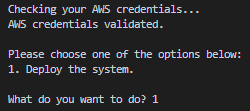
\includegraphics[width=7cm]{Resources/script_2.png}
  \caption{Action selection}
\end{figure}

\paragraph{}The deployment will then star:.

\begin{figure}[htbp]
  \centering
  \begin{minipage}[b]{0.44\textwidth}
    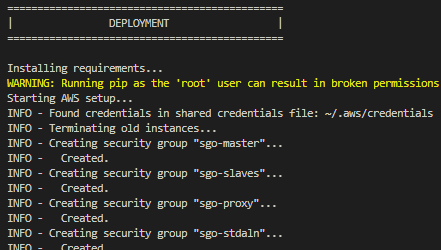
\includegraphics[height=4cm]{Resources/script_3.png}
    \caption{Start of the deployment}
  \end{minipage}
  \hfill
  \begin{minipage}[b]{0.54\textwidth}
    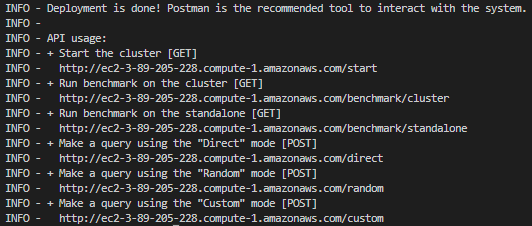
\includegraphics[height=4cm]{Resources/script_4.png}
    \caption{End of the deployment}
  \end{minipage}
\end{figure}\\

\paragraph{}The user can then interact with the REST API using any tools such as Postman. For Postman, a Collection has been included in the Github repository which gives access to all the functions of the system. Please note that the Cluster need to be start prior any other actions.

\begin{figure}[htbp]
  \centering
  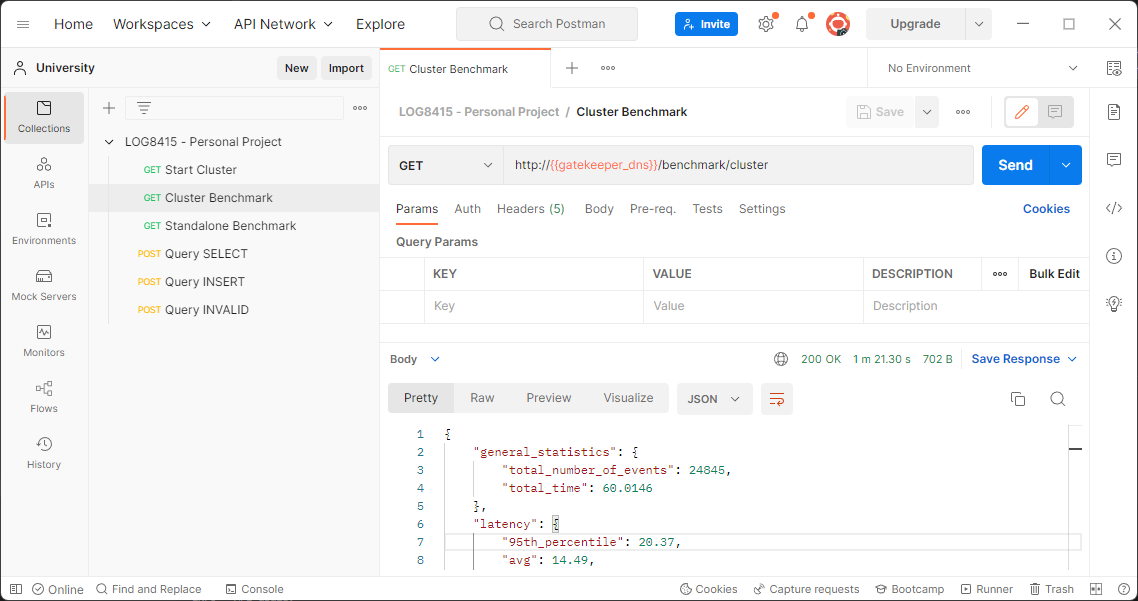
\includegraphics[width=14cm]{Resources/postman.png}
  \caption{Postman interface}
\end{figure}\\




\pagebreak
\printbibliography[heading=bibnumbered]


\end{document}
